\documentclass[a4paper,11pt]{article}


\usepackage{geometry}
\geometry{
 a4paper,
 left=30mm,
 top=30mm,
}
\usepackage[utf8]{inputenc}

\usepackage{graphicx}
\usepackage[english]{babel}
\usepackage{color}
\usepackage[dvipsnames]{xcolor}
\usepackage[colorlinks=true,urlcolor=blue,citecolor=black]{hyperref}
\usepackage{url}
%\urlstyle{same}
%\urlstyle{rm}
\urlstyle{sf}
%\urlstyle{tt}
\usepackage[font=footnotesize,labelfont=bf]{caption}
\usepackage[labelfont=it,textfont={it},singlelinecheck=on,justification=centering]{caption}
%full name for appendix
\usepackage[title]{appendix}
\usepackage{float}
\setlength{\parindent}{2em}
\usepackage{parskip}
%for code
\usepackage{listings}
%for math
\usepackage{amsmath}
\usepackage{pdfpages}
\linespread{1.1}
\setlength{\emergencystretch}{3em}

\usepackage{ifxetex,ifluatex}
\usepackage{etoolbox}
\usepackage{tikz}

\usepackage{framed}

%water mark
\usepackage{eso-pic}

\newcommand{\watermark}[3]{\AddToShipoutPictureBG{
	\parbox[b][\paperheight]{\paperwidth}{
		\vfill%
		\centering%
	\tikz[remember picture, overlay]%
	  \node [rotate = #1, scale = #2] at (current page.center)%
	      {\textcolor{gray!80!cyan!30}{#3}};
	  \vfill}}}
\usepackage{blindtext}
%water mark end


% conditional for xetex or luatex
\newif\ifxetexorluatex
\ifxetex
  \xetexorluatextrue
\else
  \ifluatex
    \xetexorluatextrue
  \else
    \xetexorluatexfalse
  \fi
\fi
%
\ifxetexorluatex%
  \usepackage{fontspec}
  \usepackage{libertine} % or use \setmainfont to choose any font on your system
  \newfontfamily\quotefont[Ligatures=TeX]{Linux Libertine O} % selects Libertine as the quote font
\else
  \usepackage[utf8]{inputenc}
  \usepackage[T1]{fontenc}
  \usepackage{libertine} % or any other font package
  \newcommand*\quotefont{\fontfamily{LinuxLibertineT-LF}} % selects Libertine as the quote font
\fi

\newcommand*\quotesize{60} % if quote size changes, need a way to make shifts relative
% Make commands for the quotes
\newcommand*{\openquote}
   {\tikz[remember picture,overlay,xshift=-4ex,yshift=-2.5ex]
   \node (OQ) {\quotefont\fontsize{\quotesize}{\quotesize}\selectfont``};\kern0pt}

\newcommand*{\closequote}[1]
  {\tikz[remember picture,overlay,xshift=4ex,yshift={#1}]
   \node (CQ) {\quotefont\fontsize{\quotesize}{\quotesize}\selectfont''};}

% select a colour for the shading
\definecolor{mygray}{gray}{0.95}
\colorlet{shadecolor}{mygray}

\newcommand*\shadedauthorformat{\emph} % define format for the author argument

% Now a command to allow left, right and centre alignment of the author
\newcommand*\authoralign[1]{%
  \if#1l
    \def\authorfill{}\def\quotefill{\hfill}
  \else
    \if#1r
      \def\authorfill{\hfill}\def\quotefill{}
    \else
      \if#1c
        \gdef\authorfill{\hfill}\def\quotefill{\hfill}
      \else\typeout{Invalid option}
      \fi
    \fi
  \fi}
% wrap everything in its own environment which takes one argument (author) and one optional argument
% specifying the alignment [l, r or c]
%
\newenvironment{shadequote}[2][l]%
{\authoralign{#1}
\ifblank{#2}
   {\def\shadequoteauthor{}\def\yshift{-2ex}\def\quotefill{\hfill}}
   {\def\shadequoteauthor{\par\authorfill\shadedauthorformat{#2}}\def\yshift{2ex}}
\begin{snugshade}\begin{quote}\openquote}
{\shadequoteauthor\quotefill\closequote{\yshift}\end{quote}\end{snugshade}}


\usepackage{listings}
\lstdefinestyle{myListStyle}{
  numbers=left,
  stepnumber=1,
  numbersep=10pt,
  tabsize=4,
  showspaces=false,
  showstringspaces=false
}

%opening
\title{\LARGE The Qitmeer White Paper:\\
	\Large The guardian of trust. The core network of the Halachain}
\author{
	Qitmeer team\\
		\small\href{mailto:paper@qitmeer.io}
			{\nolinkurl{paper@qitmeer.io}}
	}
\date{\today\\\small Version 0.1}
\begin{document}

%% Cover end
\clearpage
\pagestyle{plain}

\maketitle

%\watermark{60}{10}{hawala-network.org}

\begin{abstract}

The Qitmeer network is a blockchain infrastructure designed specifically for ....
\end{abstract}

\section{Introduction}

\subsection{Executive Summary}

Qitmeer network (Halachain,HLC) is a public blockchain based on DAG technology to serve the global Islamic economy and serve as an open, distributed ledger that can record transactions between two parties efficiently and in a verifiable and permanent way. Subject to design, HalalChain is inherently resistant to modification of the data and connects the other consortium blockchain in various jurisdictions through cross-chain protocol. 
In Halal industry it focuses on building alliance chains of traceability of halal products; And in Islamic finance industry, it mainly concentrates on developing Islamic financial products and stable cryptocurrency; All above is striving to establish an ecosystem combined with development of the underlying technologies and practical applications.
Qitmeer is building advanced blockchain based platform for Islamic economy ecosystem that will allow users investors to easily engage in the trading their ecosystem tokens using various payment methods. Qitmeer Foundation’s goal is to provide and promote the mass adoption of Blockchain technologies by becoming a globally trusted service provider. In various segment of Islamic economy ecosystem. To this end, Qitmeer have created a unique solutions with relevant regulatory compliances built into the products and services to be offered in Islamic economy ecosystem.
Today, the world has experienced half a decade of mainstream Blockchain applicable use cases, and Qitmeer are at the verge of starting  the mature enterprise blockchain era. A major strength of all Blockchain solutions revolves around their promising impact on a global financial scale. Within this context, Qitmeer strongly believe that Blockchain solutions in the global Islamic economy ecosystem which are compliant with the Shariah regulatory or enterprise technology by consumers, investors, and entrepreneurs, and as such Qitmeer is offering a flexible platform to the Islamic economy ecosystem.

\subsection{Overview of Qitmeer network}
Qitmeer network could set up a new trading platform (or move across an existing trading platform) on a blockchain protocol. Blockchain technology offers the potential to support a new medium to exchange assets without centralized trusts or intermediaries—and without the risk of double spending. As already discussed, blockchain can eliminate the threat or the risk of fraud in all areas of banking, and this could equally apply to a trading platform. Furthermore, blockchain would also address issues such as operational risk and administrative costs as it can be made transparent and immutable. The traceability and the permanent historic record that would exist on the blockchain backing up every asset or item of value that was traded, would provide assurance and authenticity all the way through the supply chain. A public chain has various performance metrics, in developing this public chain Qitmeer take into consideration various factors which are confirmation time, security including decetrialization degree and faulty tolerance threshold and high throuput. Specificly:

\subsubsection{Fast confirmation time}

Confirmation time is the waiting time when user has high confidence that a transaction being confirmed permanently, which means it can not be overun by malicious users. Confirmation time is the most important  factor in terms of user expirence, people don't have patience to bear long time confirmation. Compared to Qitmeer, bitcoin needs to wait for 6 blocks i.e. 1 hour to reach secure confirmation. Qitmeer is leveraging the fast confirmation feature in SPECTRE protocol and would be able to achive promising confirmation in order of seconds, meaning less than 1 minute, even less than 10 seconds when there is no active attack.

\subsubsection{High security}
the high security is classify into important types which 

\subsubsection{Fully decentralized}

Decentralization is the soul of a public blockchain because this is what the trust comes from for an fully autonomous system. Numbers of projects sacrifice their dectrialization to gain better throughput because of less consensus workload. This is a risky trade-off becuase less nodes to participate in consensus would bring higher possiblility to be targeted by attackers and prone to make collusion. Qitmeer's consensus protocol SPECTRE is fully decentrailized, so all nodes have full ledger and there are no super nodes.

\subsubsection{High Faulty tolerance threshold}

Faulty tolerance is refering the percentage of incapable nodes: including malicious nodes and non-operational nodes. For an autonomous network, it obeys the marjority law, so fifty percent (50\%) would be the highest standard. Qitmeer has the same 50% faulty tolerance threshold with bitcoin, so Qitmeer can provides as much security as bitcoin.

\subsubsection{High throughput}

Throughput is a repsentative metric of scalabilty, also it is a strong factor affecing practical scenarios. Bitcoin and ethereum don't scale, which have only 7 TPS and 15 TPS in theory. As a global value transfer network, such low throughput limits the vairious applications. Qitmeer is using Block DAG as our ledger underlying data structure and it could provde a conservative estimation of at least one thousand transaction per second throughput to meet most applications on blockchain so far.


\subsubsection{Methodology}

Blockchain has a big picture and Qitmeer think that it requres an architecture to undertake. The ideaology of Blockchain technology is value transfer, so this paper firstly focuses on this point and make it better than all public chains so far, then on top of that, we will extend it with much functionalities like virtual machines for smart contracts.

\subsubsection{Respect classic}

Bitcoin has various challenges so far, like scability, like centralization due to monopolized mining pools. However, most of its mechanisms are long time proved robust and promising. So Qitmeer adopted most of its classical designs, like UTXO, like Proof of work.

\subsubsection{Embrace innovation}

Qitmeer acknowledge that there is no perfect in the innovation technology, and Bitcoin is not perfect. As it just mentioned, scability and centralization, in addition, long confirmation time is also a big problem in confirming the transactions. So Qitmeer is facing these challenges and solve it with the new Block DAG protocols, SPECTRE and SPECTRE.

\subsubsection{Simple and extensible}

The scenarios in blockchain are complex and we won't solve all of them in a single complex system, which is probably unmaintainable. Instead, we design an extensilbe architect, each layer of which is simple enought to solve only a core problem. Moreover, communications are through flexible interfaces between layers. For instance, public chain is a strong foundamental value transfer network and we will make off-chain smart contracts solution on top of it. Another case is we are using block DAG to gain suffienct scalabilty for current application scenarios, since it is a leger tech, it natually could combine Sharding and layer 2 scalabilty solution to provide further scalability.

This white paper proposes an alternative to traditional applications and Blockchain solutions for Islamic Economy ecosystem and Global Islamic Financial Institutions. Currently Qitmeer public chain shall support the issuance Islamic securities (Smart Sukuk) in the Islamic capital markets industry. Instead of physical certificates/notes, Sukuk can be represented digitally in a public permissioned ledger using Blockchain in Qitmeer Smart Sukuk platform as well as other use cases for Islamic Financial Institutions.


\section{Asset Issuance Management}

There is no doubt that a high level of disruption by financial innovation has already started to reshape the global Islamic economy and the nature of payment practices; a new wave of disruption is making its way into asset management. The Qitmeer public chainblockchain records provide pseudoanonymity, as all on-chain ownership is tracked via abstract public addresses, the ownership and provenance of assets can be easily tracked and overtime particular users may be identified. While privacy may be challenging to manage, for certain applications such transparency aspects can be helpful – for example from a regulatory and compliance perspective. The Corporate entities Individuls or organizations are able to issue their assets on Qitmeer public chain platform to increase the liquility and offer finicial services. The HLc solution is reliable, user-friendly and practical especially in the Global Islamic economy and finance.

The main efforts in Islamic economics so far has been to create new forms Shariah compliance instruments to operationalise Shariah and ethical values into the current conventional economic system and financial services products. While this is crucial to sustain the global economy as it is today, the Islamic economics needs to develop new strategies to cope with the next economy, which starts with a clear and deliverable vision of a new world economy. And the new vision of a new world economy will be driven by those who embrace innovation that will build the future. 

However, it is necessary to look at the main building block to enable trust in impersonal financial transactions in a highly globalized society. This innovation called the “blockchain” will play a crucial role in boosting the Islamic financial sectors in all its segments which include banking, insurance, Capital market, Zakah and Waqf management. Addressing the digital revolution that is happening right now will foster competitive advantage for the Islamic economy and finance industry. This innovation is in accordance with Shariah rules and principles
The blockchain lets people who have no particular confidence in each other collaborate without having to go through a neutral central authority. Simply put, it is a mechanism for creating trust. Within this open ledger system, the blockchain offers an inherent level of trust for the user, eliminating the need for the middleman and mitigating the risk of human error. Justice and creditworthiness has been emphasized in the Holy Quran in Surat al Nisa which Allah says: 

O you who believe! Stand firmly for justice, as witnesses to Allah, even if against yourselves, or your parents, or your relatives. Whether one is rich or poor, Allah takes care of both. So do not follow your desires, lest you swerve. If you deviate, or turn away—then God is Aware of what you do” (4:135)

In the blockchain transaction, it is publicly accessible log of transactions ensures that the data is protected against tampering and revision, and it is virtually impossible for individuals to modify or replace parts of the blockchain secretly. The need for transparency, justice is, above all, an important Sharī`ah consideration in blockchain transaction. Any form of concealment, fraud or attempt at misrepresentation violates the principles of justice and fairness in Sharī`ah as mentioned in the Qur’an in Sūrah Al-Mutaffifin: 
Woe to the defrauders. Those who, when they take a measure from people, they take in full. But when they measure or weigh to others, they cheat. (83: 1-3)

A full copy of the blockchain contains every transaction ever executed, making information on the value belonging to every active address (account) accessible at any point in history. Every block contains a long reference number or hash of the previous block, thus creating a chain of blocks from the genesis block to the current block. The below paragraphs explain the concept of blockchain and how a transaction is recorded on the blockchain, based on the cryptocurrency protocol.
 
The Qitmeer public chain platform is one of the latest underlying technologies based on Directed Acyclic Graph which has been defined as Blockchain 3.0 technology. The DAG involves and supports quick transactions, and is friendly to small payment. This innovation shows that there is correlation between revealing civilization and blockchain consensus, which is transparency, justice, creditworthiness, trust and witness described in the Holy Quran and shared by the whole humanity. The public blockchain could act as a complete set of ecosystems to support start-ups in the Islamic digital economy and beyond. 


\section{Asset Compliance and Applicable use cases on Qitmeer}

\subsection{Qitmeer Stable Coin}

There is a contradiction between the openess of public blockchain and the compliance of assets issued on it. Blockchain is an autonomous peer-to-peer network, so there is no central authority to authorize who can join and leave. However, for a specific application scenario, Qitmeer have to make sure that the assets issued on Qitmeer public chain platform are compliable with Shariah law principles. It is mentioned that innovation is important as the humanity are living in the age of technology and in an era of extreme innovation; with every passing day human being are harnessing new possibilities and existing opportunities using technology. Nowadays, one of the most talked-about topics in the financial services industry is to enable Capital markets, money markets and banks to process payments more quickly and more accurately while reducing the costs of processing transactions. However, The technology could be adopted in the area of Stable coin, sukuk, takaful, banking, waqf, zakat,etc.

\subsubsection{Qitmeer Stable Coin Definition}

A stable coin is a currency which successfully performs its functions as a means of exchange, unit of account and a store of value because its purchasing power is stable. but is not tied to a central bank and has low volatility. On any given day, it is common to see an increase to 10-20% or even a decrease. That makes using most cryptocurrencies for daily transactions inconvenient. The adoption of stable currencies/coins will be a catalyst to the new decentralized internet becoming mainstream.
Stable coins is  core product is a Shariah compliant smart contract that represents an equity stake in Sukuk portfolio, which successfully combines traditional Islamic finance principles with those of mainstream finance. Stable Coin is a token whose smart contract represents the owners’ share in a financial fund formed by investment grade Sukuk. When consumers purchase the token, they are buying in to a fund of diversified Sukuk of high quality and high liquidity Sukuk.


\subsubsection{Features Of The Qitmeer Stable Coin}
 
Currency and  Security As a currency, Qitmeer is a system that enables payments settlement between two parties, directly, without the need of a central party to monitor transactions. Also, as a security, Qitmeer is backed by investment grade Sukuk that allows the token to not only remain stable, but steadily appreciate in value, making it ideal as a savings instrument. Qitmeer carries divisibility, homogeneity, portability and stability due to its asset-backed nature.

\textbf{Equity and Debt}

As a token, Stable Coin represents an owner’s equity stake in a financial fund that is comprised of investment grade sukuk. We estimate that this fixed-income product will, return between 3-7% for retail investors, which is the average range for high quality sovereign and private Sukuk issuance. At the peak of its development, Fasset will also be able to support the raising of Shariah-Compliant debt for both corporates and sovereigns through its wider community of retail and institutional investors.  

\textbf{Stability}

The final feature of the coin is in its stability. Backed by a real asset, the coin will not be subject to huge variations in price and thus will in effect become a form of stable coin. Coins will be issued 1:1 against the value of the Sukuk fund.

Insert Diagram or Table here

\subsubsection{Applicable uses of Qitmeer Stable Coin}

The use of Blockchain technology holds great potential across the Islamic economy and finance industry. One of the key principles of Islamic economy is based on having enforceable contracts which are fair, transparent and agreeable between the parties that engage in a banking transaction.

\textbf{Payments}  
As a currency, Stable currency can be a payments system for goods and services. The Shariah-compliance and homogeneity offered by Qitmeer can form as a reliable and low cost payments settlement vehicle for SMEs and large companies. 

\textbf{Transfers}
Our ecosystem will provide the infrastructure for an instantaneous international transfer system. The stability, portability and real world liquidity of Fasset will allow for fast, cost-less remittances across borders – especially given the fact that the Fasset ecosystem will be built on the DAG protocol (see Section 3: Technology Context for more information).  

\textbf{Savings} 
As of now, retail customers are unable to access the Sukuk market for long term savings - Qitmeer will democratize access to a Shariah compliant fixed-income investment fund for retail consumers. The fixed-income nature of Sukuk and the divisibility offered by Fasset will allow retail investors to transfer their savings into Fasset for safe, secure and steady returns. 

\textbf{Liquid asset} 
Stable Coin can replace commodities such as copper that are required for debt based Shariah financing. Thus, Qitmeer can accommodate many real-life transactions, for instances al Murabahah, Tawarruq, etc. 

\textbf{Liquidity management}  
Perhaps the most important use case for the Qitmeer ecosystem will be in playing a vital role as a much-needed and oft-requested secondary market for the Islamic Finance industry. The speed, security and cost savings from encoding smart contracts using distributed ledger technology will provide strong options for liquidity management. This will enable numerous functions that have so far stalled the growth of Islamic Finance – such as inter-bank lending, monetary supply management by central banks and in enabling the development of other bespoke Shariah compliant institutional products.

\section{Smart Sukuk on Qitmeer public chain}

One important application in Islamic capital markets for blockchain is the sukuk (Islamic bonds) market. Sukuk are securitized, and hence tradable on secondary markets much like a stock can be traded on a stock exchange. Islamic finance prohibits interest payments on loans and the sale of debt; Sukuk markets evolved to securitize Islamic modes of financing such as profit sharing through asset ownership for a given tenure.

Sukuk has been a popular approach for governments seeking to finance infrastructure projects, but the legal complexity and overall cost to issue sukuk has kept it out of reach for smaller corporations and MSMEs. It has been an excellent way to raise much needed capital, but investors have also been always restricted to the much larger institutional investors due to the high barrier of entry, which usually starts in the millions. However, the inability to lower these barriers of entry at the retail level to thousands or hundreds of dollars to enable wider participation (and access to more funds) for sukuk participation, and hence wider risk and profit-sharing in the Islamic capital market, is still persistent and remains an impediment to true shared prosperity.

\subsection{Sukuk investment: An Ethical Investment For  Stable  Returns}

According to IFSB 9 (IFSB, 2007) Sukuk commonly refers to the Islamic bonds. However, as opposed to conventional bonds, which merely confer ownership of a debt, Sukuk grants the investor a share of an asset, along with the commensurate cash flows and risk. As such, Sukuk securities adhere to Islamic law, referred to as Shari’ah principles, which prohibit the charging or payment of interest.

Put simply, Sukuk instruments act as a bridge. They link their issuers, primarily sovereigns and corporations in the Middle East and Southeast Asia, with a wide pool of investors, many of whom are seeking to diversify their holdings beyond traditional asset classes. In this way, funds raised through Sukuk can be allocated in an efficient and transparent way to infrastructure initiatives and other deserving projects linked directly to the real economy sector.

Development of Traditional Sukuk market 2017 ended on an optimistic note for the global Sukuk market. There were relatively higher commodity prices (particularly of oil), a gradual rise of reference rates, and a marked increase in Sovereign Sukuk issuances, stable Corporate Sukuk issuances in certain jurisdictions and a healthy Sukuk issuance pipeline. Sukuk continued to gain attention from new issuers while the investor base expanded, which is an encouraging development. During the year, Sukuk were issued as a viable alternative source of financing for infrastructure development, aircraft financing, project financing, corporate general purpose needs, capital adequacy and budgetary requirements. Other interesting developments are the issuance of Green Sukuk and increased interest in SRI Sukuk issuances.

The year’s landmark event was Saudi Arabia’s entry as a sovereign Sukuk issuer. The country’s first issuance was the largest international Sukuk issuance ever of USD 9 billion, followed by several sovereign domestic Sukuk issuances. The other new sovereign issuer was Nigeria with the country’s domestic issuance being around USD 312 million. In addition, continued interest from well established sovereign, quasi sovereign and financial institutions issuers such as the Governments of Bahrain, Indonesia, Turkey, Pakistan, Oman, Hong Kong, Investment Corporation of Dubai, and Islamic Development Bank has kept the Sukuk market active. New issuers, such as Saudi Arabia, have helped keep the growth trajectory of Sukuk issuance intact.

\subsection{Global Sukuk Issuances}

Total global issuance amounted to USD 116.7 billion in 2017. As illustrated in Chart 1 below, global Sukuk issuance has increased from USD 87.9 billion in 2016 to USD 116.7 billion in 2017, an impressive jump of around 32% in volume. The increase in volume during 2017 was mainly due to sovereign Sukuk issuances by Saudi Arabia coupled with steady issuances from Asia, GCC, Africa and certain other jurisdictions. Malaysia continues to dominate the Sukuk market, though shares from countries like Indonesia, the UAE and to some extent from Turkey, are close behind in value.

                                              Insert Diagram or Table here

Sukuk - has thus far been limited to governments and large institutions due to the high issuing costs and complexity. But there is new approach and innovation in Islamic Economy from Qitmeer perspective aims to using the blockchain. Using blockchain technology can solve most of the Shariah and legal  issues in the Sukuk issuance. Islamic Securities can be executed according to predefined rules can be coded as a smart contract in capital markets. 
Experiments are ongoing on the issuance of smart bonds. Sukuk issuance follows strictly Shariah law and principles of permissible variance, cleansing, the balance-sheet ratios to be satisfied, the 'conglomerate' issue and the 'core' activities. The following Table shows the traditional Sukuk.
Insert Diagram or Table here
These Smart Sukuk can also be coded as if-then statements to ensure both compliance to the Shariah and transparency for all involved. This would increase the investors satisfactions on the Shariah compliance of Sukuk product.
Smart Sukuk standardizes and automates much of the legal, accounting, and payment overhead of conventional sukuk offerings - all backed by fully licensed legal entities in the issuing jurisdiction.

\subsubsection{Smart Contract and Blockchain}

The role of smart contracts in the smart Sukuk.  A smart contract is a piece of code within a blockchain record that is executed by each node on the network to automate (potentially) a particular state resulting from a contractual deliverable without further human interaction. For example, in the context of a loan or a bond you could put in place a smart contract at the time of issue that automates the payment of interest to each investor on the given due dates. Accordingly, the bond or loan would service itself when triggered by the borrower sending funds to the smart contract. It is therefore a very useful tool to automate operative parts of normal legal contracts, but all the regular contractual protections such as representations, warranties and indemnities drafted in natural language are still needed. These cannot currently be replaced with code It’s fair to say there is some confusion and concern about smart contracts among lawyers with many concerned that regular natural language contracts will be replaced by code. This is not currently viable or realistic. Smart contracts are not a replacement for normal legal contracts but rather sit behind and augment a legal contract where by snippets of code replicate and automatically perform certain terms of the contract.

The Investors in a sukuk are issued a share of ownership, which represents their fractional ownership in the underlying asset or structure with the terms of the sukuk ownership. Holders of sukuk receive periodic payments from the fund-raising institution. Investors can hold a sukuk until maturity, or they can sell their ownership in the sukuk to a third party. This subsequent sale to a third party is known as “secondary trading” and is what distinguishes a sukuk as a “securitized” asset.
Smart Sukuk runs on the Qitmeer public chain, which supports “smart contracts”. A smart contract encodes business rules directly into the underlying payment currency itself – the blockchain itself enforces the contract rules regarding payments and transfer of ownership.

\subsubsection{Smart Sukuk Definition} 

The experimental bond was also issued by Fasset  through Qitmeer’s public chain platform, but this is new  denominated in ether. As such, it will be the first ever cryptocurrency Sukuk fully settled on an open public blockchain using smart contracts. While cryptocurrency Sukuk have been issued under crypto asset conditions, and there have been some bonds issued where payment has been made in cryptocurrency, this was the first time a Sukuk has actually been denominated in cryptocurrency, fully settled on a blockchain and issued on a commercial basis by a trading company in a regulated way. It is significant because HLC foundation will able, for the first time, to issue and pay for a legally enforceable financial instrument without using any of the traditional existing financial infrastructure.
Smart Sukuk, can be defined as tokenization by collecting funds from investors in exchange for Sukuk Tokens representing an ownership portion of the Sukuk investment. When the institution makes payments, the funds are automatically distributed back to the Sukuk Token holders via the blockchain according to the rules of the smart contract in Islamic Economics - without the need of conventional banks or intermediaries.
Smart Sukuk is where the investors transferred Ether from their existing blockchain wallets, such as a Coinbase account, to their Qitmeer cryptocurrency wallets. On settlement, ether passed from investors’ cryptocurrency wallet addresses to Fasset’s address, and the Sukuk passed from Fasset’sIslamic securities wallet address to the investors’ addresses. All of this is recorded on the public blockchain technology and represented through the Qitmeer public blockchain interface on the HLC platform. 
                                    Insert Diagram or Table here

From a Islamic securities perspective, the blockchain served as the register and denoted legal and beneficial ownership. Because the Financial Authority recognised the blockchain as an independent third party, there was no need for a registrar to keep a register of Sukuk holders: the register is the blockchain. Smart contract code was put in place behind the regular legal contracts to automate delivery of the Sukuk and payment flows, so Fasset issued the smart Sukuk and paid investors’ returns and principal automatically, without further action.
Smart Sukuk Tokens support an industry standard protocol, called ERC20. The standard allows tokens to be traded globally on a variety of public cryptocurrency exchanges.

\subsubsection{Structure of Smart Sukuk}

Islamic Economics and finance is bound by Shariah rules and regulations from the regulatory authorities. The Qitmeer token and other Cryptocurrencies in Islamic Economy is permissible based on its attributes and underlying asset which is Qitmeer commodity. The Halalchain will offer the Smart Sukuk in jurisdictions with clear and viable legal and regulatory frameworks to support the issuance of Smart Sukuk. 
The structure of the Sukuk above will be base on Sukuk Ijarah and hybrid Sukuk projects “Take Sukuk al-ijarah (lease based) as an example – an Sukuk ijarah is permissible and Shariah compliance if the true ownership of the underlying asset is legally transferred to the Sukuk holders. And for a Smart Sukuk, it’s only acceptable because of its regulation on trading and exchange in the Cryptocurrency Assets.”
Smart Sukuk supports issuance of the sukuk in global/local currencies and eliminates the need for institutions to add cryptocurrency to their balance sheet. The use of blockchain allows for legal and beneficial title to be united. This meant that the global/definitive note structure that underpins most Islamic securities issuance was dispensed with, removing a lot of the detailed language that first-time issuers often struggle with.

\subsubsection{Features of Smart Sukuk}

The adoption of stable currencies/coins will be a catalyst to the new decentralized internet becoming mainstream. Sukuk issuance on Blockchain simplifies Islamic securities issuance and reduces cost in a number of ways: .

Firstly, it means legal fees and complexity are both lessened because the documents and structure are simpler. As described above, the use of   blockchain allows for legal and beneficial title to be united. This meant that the global/definitive note structure that underpins most securities issuance was dispensed with, removing a lot of the detailed language that first-time issuers often struggle with. 

Secondly, the absence of a registrar meant that the normal contractual relationships that needs to be created between issuer and registrar could be dispensed with, and the issuer does not need to pay a registrar to perform the function. Thirdly, payments could be made on a peer to peer basis ie the issuer pays interest and principal directly to investors automatically via the use of smart contracts. Accordingly, there was no need to have a paying agent, which again reduced the complexity of the documentation and also meant that the issuer did not need to pay a large bank to fulfil the role. Finally, on the investor side, the ease with which someone can open a blockchain wallet means that there is less need for a long chain of custody.

As a result there were fewer parties involved and substantially shorter and less complex bond documents. This reduces the cost and time to market for issuers and it should be clear from the structure diagram below how much simpler this is than the traditional structures described above.
It is important to note that any party can independently verify the allocation of cash and assets on the blockchain without using HalalChain’s system. This is important, because if the system were to fall away for any reason, the contracts could still be enforced as between holders and the issuer. Enforcement would work in much the same manner as a regular bond issuance. For this issuance Link acted as trustee so if there were to be an event of default then holders would be able to enforce their rights via the trustee in the usual fashion and ultimately through the courts. On an issuance without a trustee, bondholders would be able to enforce rights directly. Smart contracts do not change or diminish enforcement rights, there were still regular legal contracts that any capital markets lawyer and the courts would recognise, and understand.

\subsubsection{Waqf Chain Endowment}

In the Islamic Finance, there is a particular opportunity in Waqf’s tremendous potential and development. For decades, the administration of Waqf assets has been a challenge in Islamic Economics and finance. Billions of Waqf funds/assets globally that could be used to education and alleviate poverty, are simply not being utilized efficiently. However, the advent of blockchain technology has brought hope and optimism to Waqf administrators and Shariah scholars in Islamic Economy. 
In 2010, Ernst \& Young estimated the global WAQF sector to be worth over US 105 billion. Informal estimates by experts suggest that Waqf assets could be as high as SAR 1 trillion (US266.6) in Saudi Arabia alone, while in Malaysia, Waqf assets have been estimated at RM1 trillion (US325.4 billion), and in Egypt a recent report by ministry of Religious Endowment estimated Waqf endowments of around US 82 billion. Qitmeer has identifies endowment as an underserved market niche commensurate with its vocation to be the social Solution for Blockchain.

                                           Insert Diagram or Table here

With the use of continuous innovations and disruptions happening in the financial and technological, Islamic economics, including Waqf principles are being forced to maneuver and reinvent themselves, especially in terms of governance and regulations so as to remain relevant since they constitute a major socio economic institution in the modern financial market. 
Qitmeer intends to provide a smart contract ecosystem and accompanying blockchain to allow Waqf boards and other interested stakeholders the opportunity to submit project outlines/plans in order to fund and develop projects on top of Waqf properties. 
Qitmeer will develop a specific interface for this selected asset. Contributors will then be able to select, visualize and assess those properties before deciding on their contributions to their development.
hese contributions will be made possible through token or other means and will include the possibility for various purpose and interests depending on funders’ expectations. Specifically contribution as charity , Waqf investments or Islamic bonds all are intended to be integrated. Each project will have its own attached digital token under the Qitmeer coin standard. This token will be placed into a project crowdfunding smart contract that can only be started once the project has passed all due diligence requirements.
After the crowdfund has been completed, any resulting project tokens are claimable by participants, these tokens are digital assets representative of a participants stake in that project. The following diagrams show the various stakeholders and institutions involved in executing and delivering a Waqf property project along with the flow of funding and project development.



\subsubsection{Value relevance}
The assets issued on Qitmeer public chain All the current assets issuance platforms, like ethereum, don't have a threshold to issure assets. So people could create assets whatever "market value" they want. Firstly it makes users hard to tell which asset is valuable or just a spam; secondly, abuse issuance increases the computation load and finally user will have to pay for it in the form of transaction fees.
 (what is difference between asset relevance and value relevance, it is possible to merge it?)


\subsubsection{Asset compliance}
The challenges of asset compliance is that the current solutions don't seperate application governance from consensus. Public blockchain itself is just a temper-proof ledger or database, so it is able to provide trustful computation services, which means the service will deliver what its code promises, so we could deem it as a technology problem. However, application governance is a bussiness problem and should be managed by the users rather than miners or developers. 

\subsubsection{Asset relevance}
The cause of asset relevance problem is that the value of asset (tokens) and underlying currency (coin) don't  enter in a unified ecosystem. For instance, some token could be no connection with the ETH coin. In theory, this problem cannot be solved because we cannot estimate the market value of one toke, however, at least we should offer a benign mechanism that make tokens related to the coin, so it will encourgae the issuer to devote more value to gain more their customer's trust.



\section{Smart Islamic Banking on Qitmeer network}

Smart contracts on the blockchain could and will create efficiencies and therefore savings for every category of monetary markets, investments, Banking and other financial services like insurance/takaful but more important, they will reorganize how certain services are run within the economy. To illustrate this, the paper focuses on some financial service areas like banking, which could benefit from immediate sizeable savings:

Islamic Banks need to adopt Blockchain technology to transform sizable chunks of their business. This technology’s aim is to change the normal conventional banking by making it easier and simpler for everyone to perform banking activities from anywhere regardless of their social status. Blockchain is a disruptive technology that will fundamentally change banking as well as many other industries. Blockchain presents a two-fold solution for Islamic banks. One, it could potentially save banks billions in cash by dramatically reducing processing and transaction costs; and two, the reduction in the amount of time and the amount of paper that they process. Implementing Blockchain would make banks increasingly profitable and valuable.  The Islamic financial sector has experienced substantial developments in the new century and has grown very rapidly both in size and number of institution. With this requirement, Islamic banking has been continuously developing new Shariah compliant products that both alter their ability to compete with conventional banks and alter their risk taking and risk mitigation profile. 


\subsection{What is Smart Islamic banking}

What is Smart Islamic banking refers to a system of banking or banking activity that includes financing and investment without interest that is consistent with the principles of the Shari’ah. An Islamic economic principle offers a balance between extreme capitalism and communism. It has the same purpose as conventional banking except that it operates in accordance with Shari’ah rules and principles. The Islamic banking is design on two main basic principles; one is collection and payment of Interest (Riba) is not allowed, which means their model is based on sharing of profit and loss concept; and the second, the bank cannot create any debt without goods and services to back it. Hence savings, deposits and investments mostly with the Islamic Bank will be backed by physical assets.
The smart Islamic banking will facilitates automatic payment processing, only if certain parameters within the agreed upon contract are satisfied. Because of smart contracts, costly errors from the manual processing of contractual terms, including settlement instructions, can be reduced considerably. If an American bank has transacted a trade or swap contract with a GCC bank, the settlement details would only be provided if the financial details of the trade match between the two banks. 

\begin{itemize}
    \item Trade finance like supply-chain documentation, invoicing, and payments in letters of credit, trust receipts, etc. 
    \item Mortgages for housing. The mortgage loan process relies on a complex ecosystem for the origination, funding, and servicing of mortgages, with considerable costs and delays. 
    \item Loans without interest of any kind, including crowdfunding for start-ups and small and medium-sized enterprises (SME). Distribution of equity of micro, small, and medium-sized enterprises (MSMEs) to investors.
The global financial crisis has failed to have more impact on Islamic banking as compare to conventional banking system, and they remain stable at the early phases of the global financial crisis. The main reason is their banking principles, its transparency and assets back financing, which did not permit speculative economic activity.
\end{itemize}

\section{Smart Takaful on Qitmeer network}

As a niche section of the insurance sector, the takaful segment is significantly impacted by the disruptions occurring within the insurance sector. The global insurance market had a reasonable growth rate, with global real premium growth rates of 2.9% in the advanced economies and 7.4% in the emerging and developing countries in 2014, an improvement over the 2012 and 2013 rates (IFSB, 2016). Likewise, the growth rate of gross contributions in the takaful sector demonstrated a recovery in 2014 from 2013, when the growth rate of premiums was by far the lowest historically.
Takaful is a system of Islamic insurance based on the principle of mutual cooperation and donation (Tabarru), where the risk is shared collectively and voluntarily among the participants. Takaful claims, is a distributed process that involves many parties, participant, Takaful Operator and beneficiary, often with insufficient transparency to the participants. 

Smart contracts deployed through the blockchain will provide customers and takaful (insurance) Operators a system to manage claims in a transparent, quick, and indisputable manner. Takaful policies, along with its terms and conditions, and potential claims can be recorded onto the blockchain and validated by the network, ensuring valid claims are dispensed and false claims are rejected.  For example, the blockchain will reject multiple claims for one accident because the network would know that a claim has already been made. Smart contracts would also process claims efficiently by triggering payments automatically when certain conditions are met and validated. To more effectively detect identity fraud, falsified injury or damage reports, etc., blockchain can be used as a cross- Islamic Financial Institutions (Islamic Finance industry).

\subsection{What is Smart Takaful}

Takaful claims processing and settlement, are areas where participants make a contribution and the Takaful operator sets out rules under which, the participant gets a coverage. The level of expertise required for claim adjusters or the investigators, who investigate, negotiate and settle claims, varies directly with the nature of loss, under the jurisdiction whose law applies to the contract creation, interpretation and enforcement, one of principal consumer protection issues within the Takaful pricing, underwriting, and claim settlement process, the rules-based claims processing or otherwise a voting based claims processing, mostly followed by mutual agreement. 

The settlements are also subject to interpretation of the rules that apply to the product and participant situation. This leads the claim processor to apply rules and make decisions before paying out the claim. Storing and reconciling data sets of financial obligations and ownership forms are the core of Takaful claims operations. The current methods are highly complex, use fragmented IT and data architectures and suffer from a lack of common standards. This creates a continual need to reconcile data with massive systems and process duplication, leading to high costs and protracted time to execute tasks. Block-chain can be used to manage shared intelligence and could be used to drive efficiency in Takaful claims processing independent of fraud, thus bringing a structural change to the industry. 
Further, in lines of Takaful where losses require onsite examination, claims adjusters may be sent to conduct an investigation. Takaful smart claim (TSC), through the block-chain-based systems could help radically improve the Takaful company operations in term of efficient claim processing and settlements, claims adjusters' investigation and decisions on which claim should be paid, with the means to manage claims in a transparent, responsive and irrefutable manner. These features or innovation could be built into the Takaful existing market infrastructure in making the claim, it would allow for the auto-execution of coded logic embedded into smart claims.

The block-chain lets people who have no particular confidence in each other collaborate without having to go through a neutral central authority. Simply put, it is a mechanism for creating trust. Within this open ledger system, the block-chain offers an inherent level of trust for the user, eliminating the need for the middleman and mitigating the risk of human error. Thus, it promotes justice and creditworthiness which has been emphasized in the Holy Quran in Surat al Nisa (4:135)

In this innovation, block-chain transactions can be a reversed engineered to allow a pretty good guess at the transactor. Another block-chain virtue is the decentralization of customer databases and a federated identity infrastructure that allows an individual to identify information online without having to supply personal information (for example, a driver’s license number to multiple Takaful operator). Rather than being held in any number of central databases, sensitive data is encrypted and distributed and a block-chain is used as an audit ledger to re-authenticate the user. 

                                    Insert Diagram or Table here


This Smart Takaful will help the Takaful operator to record transactions on a block-chain at each point in the transactional lifecycle, from seeking a quotation to binding contract, the immutable life record of that contribution of participant can be traced. This does bring a degree of simplicity to the underwriting process and has the potential to reduce fraud. The main purpose of Takaful is to provide assistance to the participants when they are in any difficulties or losses, such mutual assistance will be significantly achieved by the means of automated Takaful claim processes that are efficient, transparent, faster, cheaper and more secure by adopting block-chain technology.

Within claims prevention, new data streams can enhance the risk selection process by combining location, external risk and analytics. A distributed ledger can enable the TO and various participants to easily and instantly access and update relevant information (e.g., claim forms, evidence, police reports and third-party review reports). 

The use of data from a mobile phone or sensors can streamline claims submission, reduce loss adjuster costs and increase customer satisfaction, with block-chain systems facilitating communications and coordination among all parties. Consider how sensors can trigger alerts to TO that a crash has occurred (thereby initiating a new claim), and then route secure and relevant data to preapprove and conveniently locate medical teams, towing services and/or repair garages. Here again, block-chain is the network connecting and ordering data from the multiple devices and apps involved in the multidimensional process. 

This Smart Takaful will help the Takaful operator to record transactions on a block-chain at each point in the transactional lifecycle, from seeking a quotation to binding contract, the immutable life record of that contribution of participant can be traced. This does bring a degree of simplicity to the underwriting process and has the potential to reduce fraud. The main purpose of Takaful is to provide assistance to the participants when they are in any difficulties or losses, such mutual assistance will be significantly achieved by the means of automated Takaful claim processes that are efficient, transparent, faster, cheaper and more secure by adopting block-chain technology.

\section{Qitmeer Token Design}

The HLC public chain is a powerful innovative technology that has the potential to transform the global Islamic financial services industry. it is a distributed database of records or public ledger of all transactions or digital events that have been executed and shared by corporate entities. HLC technology is cryptographically authentacated. it is developed to provide an alternative secure approach to exchange value without the involvement of third party. The technology enables simplification and brings in greater security, scaleability, speed, and reliability. The results is reduced costs and improved efficiency. 

\subsection{Overview}

the $\texttt{OP\_TOKEN}$ is inspired by Color coin idea, which representing and managing real world assets on top of the Bitcoin by using $\texttt{OP\_RETURN}$, and the OP\_GROUP, a referenced implementation of issuring assets designed by Andrew Stone.

the OP\_TOKEN fit various practical scenarios with unique features like asset compliable and value relevent. There are some related concept in the details below:  

\subsubsection{UTXO}

UTXO represents Unspent Transaction Output. One transaction has multiple sources and destinations, we call them as inputs and outpus. There are no accounts in HLC, what users have and spend are a bunch of unspent transaction ouputs and we could get  balance by summing up them. 

\begin{figure}[hbt]
	\centerline{%
	   \resizebox{0.8\textwidth}{!}{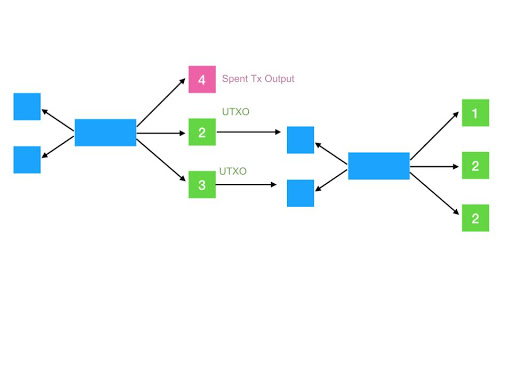
\includegraphics{figures/utxo-1.jpg}}%
	}
\caption{utxo model}
\end{figure}


The first transaction tx1 has 3 outputs and the first output of them is spent, so  tx1 has 2+3=5 coins balance. 

The second transaction tx2 spends the 2 UTXOs of tx1 and pays to 3 addresses and creates 3 new UTXOs. 

Note: now the old UTXOs (of tx1) are no longer UTXO so cannot be spent later.  

\subsubsection{Script system}

The mechanism behind how users spend their UTXOs is to execute a special script. The output stores a half of the script and we have to present the other half and combine both to verify if we could spend the money. The former half is called locking script, like a locked treasure box, and the latter is unlocking script, like the only key to the box.

Let's take a look at the typical instance of  Pay-2-Public-Key-Hash(P2PKH)

Locking Script in UTXO:

\begin{lstlisting}
OP\_DUP OP\_HASH160 <PUBLIC\_KEY> OP\_EQUALVERIFY OP\_CHECKSIG
\end{lstlisting}

Unlocking Script in a newly created transaction:

<Signature><PublicKey>

Combine unlocking script with locking script:

<Signature><PublicKey> OP\_DUP OP\_HASH160 <PUBLIC\_KEY> OP\_EQUALVERIFY OP\_CHECKSIG

This whole script consists two steps
1. <PublicKey>  OP\_HASH160 <PUBLIC\_KEY> OP\_EQUALVERIFY
	To very if the public key in the unlocking script matches that in the locking script.
2.  <Signature><PublicKey> OP\_CHECKSIG
	To check if the signature is valid.


\subsubsection{Color coin and USDT}

Color coin is a method to represent assets on top of the blockchain, so it can leverage the temper-proof capibility of blockchain. It use tx-script operation $\texttt{OP\_RETURN}$ to interupt script execution early, so we can add information of the assets after it without violating the script validation.

Locking Script:
\begin{lstlisting}
OP_RETURN <DATA>
\end{lstlisting}

The stable coin Tether (USDT) also uses OP\_RETURN based omni layer protocol to define the asset on the bitcoin. 

Here is a typical USDT transacation and details of its protocol design


\lstset{basicstyle=\tiny,style=myListStyle}
\begin{lstlisting}
OP_RETURN 6f6d6e69000000000000001f00000015c9054900
\end{lstlisting}


\begin{figure}[hbt]
	\centerline{%
	   \resizebox{0.8\textwidth}{!}{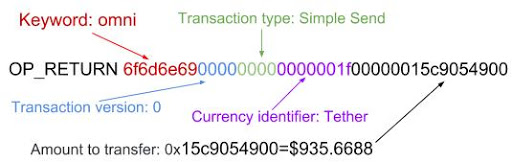
\includegraphics{figures/usdt.jpg}}%
	}
\caption{usdt}
\end{figure}


%[ref][https://www.blockchain.com/btc/tx/efc50d9e1f23e687e304cfca4ef2c5412b67d5737888ff80a0cbb6853cd865c]



\subsubsection{OP\_GROUP}
The OP\_RETURN scheme is more suitable to apply on mature blockchain since it doesn't change the underlying blockchain protocol and won't risk forking. However, the weakness  is that miners cannot verify its protocol so there would be some security risks.

OP\_GROUP is a proposal of assets issuance  on Bitcoin Cash (BCH) from Bitcoin Unlimited (BU) and has been approved by BU. OP\_GROUP supports token issuance, tranfer, destroy, etc. Since OP\_GROUP is an extention to BCH script sytem,  it is part of BCH protocol and can be verified by miners, which is more reliable.

The basic “colored” pay 2 public key hash script would be like: 

\lstset{basicstyle=\tiny,style=myListStyle}
\begin{lstlisting}
OP_DATA(group address)  
OP_GROUP  
OP_DROP  
OP_DUP  
OP_HASH160  
OP_DATA(pubkeyhash)  
OP_EQUALVERIFY  
OP_CHECKSIG
\end{lstlisting}

The main difference is simple, just adding a group address to distiguish different groups, and the other operations ,such as create and destroy assets, are similar.

% [ref]https://medium.com/@g.andrew.stone/bitcoin-scripting-applications-representative-tokens-ece42de81285

\subsection{OP\_TOKEN Design}

\subsubsection{Overview}

There is a special token named LICENSE in OP\_TOKEN. Licenses are held by renowned expects or organizations with public credibility. Any entitity planing to issue a token needs to be warranted a license. Since license is also a token, it is able to be transfered between peers. However, license transfer can be tracked through transaction history, so the originator would be very cautious in case transfering to a wrong hand.

\subsubsection{Issuance of License}

Licenses are all generated in genesis block and distribted to 100 preserved committe members. One smallest unit of HLC (SAND) represents a license,  one block has 100 HLC,  1 HLC= 10\^8 SAND , so we have 10 \^10 license in total, which is sufficient for asset issuance.


\lstset{basicstyle=\tiny,style=myListStyle}
\begin{lstlisting}
INPUTS:
	INPUT:
		PREVIOUS_OUTPUT: # (COINBASE of GENESIS)
		SCRIPT: "DUP HASH160 [GENESIS_HASH] EQUALVERIFY CHECKSIG"
		VALUE: 10000000000 (10 billion)
		SCRIPT: "[SIG] [GENESIS_PK]"
OUTPUTS:
	OUTPUT:
		SCRIPT: "[LICENSE_HASH] TOKEN DROP DUP HASH160 [COMMITTEE_1_HASH] EQUALVERIFY CHECKSIG"
		VALUE: 100000000 (100 million)
	# ... ... (COMMITTEE 2~99)
	OUTPUT:
		SCRIPT: "[LICENSE_HASH] TOKEN DROP DUP HASH160 [COMMITTEE_100_HASH] EQUALVERIFY CHECKSIG"
		VALUE:100000000#(100 million)
	OUTPUT:
		SCRIPT: "RETURN [DATA]" 
		VALUE: 0
\end{lstlisting}


\subsubsection{Warrant a license}

The individual and corporate entities/companies must be warranted a license to issue assets. These companies can request license from any committee member. Once the license is granted and approved, it would receive a special token transfer from the commitee member and the token is the license.

\lstset{basicstyle=\tiny,style=myListStyle}
\begin{lstlisting}
INPUTS:
	- INPUT:
		PREVIOUS_OUTPUT:
			SCRIPT: "[LICENSE_HASH] TOKEN DROP DUP HASH160 [COMMITTE_HASH] EQUALVERIFY CHECKSIG"
			VALUE: 100000000
		SCRIPT: "[SIG] [COMMITTE_PK]"
OUTPUTS:
	- OUTPUT:
		SCRIPT: "[LICENSE_HASH] TOKEN DROP DUP HASH160 [ISSUER_HASH] EQUALVERIFY CHECKSIG"
		VALUE: 1
	- OUTPUT:
		SCRIPT: "[LICENSE_HASH] TOKEN DROP DUP HASH160 [COMMITTE_HASH] EQUALVERIFY CHECKSIG"
		VALUE: 99999999
	- OUTPUT:
		SCRIPT: "RETURN [DATA]" 
		VALUE: 0
\end{lstlisting}

\subsubsection{Issuance of assets}
Once warranted a license, organizations are able to issue assets. Assets cannot be built from the air, they required equal amount smallest unit (sand) of HLC to be converted. This process is called as "token mint". it is like to mint a gold coin requires the same weight of gold sands, tokens need same amount of HLC sands. The advantage is not only that the token has a value support by underlying currency but also that all tokens and HLC are invovled in the same ecosytem, which would improve the liquidity and make whole network healthier.

\lstset{basicstyle=\tiny,style=myListStyle}
\begin{lstlisting}
INPUTS:
	- INPUT:
		PREVIOUS_OUTPUT: #(1 LICENSE)
			SCRIPT: "[LICENSE_HASH] TOKEN DROP DUP HASH160 [ISSUER_HASH] EQUALVERIFY CHECKSIG"
			VALUE: 1
		SCRIPT: "[SIG] [LICENSE_PK]"
	- INPUT:
		PREVIOUS_OUTPUT: #(1 HLC)
			SCRIPT "DUP HASH160 [COIN_HASH] EQUALVERIFY CHECKSIG"
			VALUE: 100000000
		SCRIPT "[SIG] [COIN_PK]"
OUTPUTS:
	- OUTPUT:
		SCRIPT: "[LICENSE_HASH] TOKEN DROP DUP HASH160 [ISSUER_HASH] EQUALVERIFY CHECKSIG"
		VALUE: 1
	- OUTPUT:
		SCRIPT: "[TOKEN_HASH] TOKEN DROP DUP HASH160 [PK_HASH] EQUALVERIFY CHECKSIG"
		VALUE: 100000000
	- OUTPUT:
		SCRIPT: "RETURN [DATA]"
		VALUE: 0
\end{lstlisting}

\subsubsection{Transfer of the Assets}

Assets can be transfered between parties. Moreover, we could transfer mulitple assets within one transaction. The transaction needs to ensure the  input sum of each asset equals the output sum of each asset. 

\lstset{basicstyle=\tiny,style=myListStyle}
\begin{lstlisting}
INPUTS:
	- INPUT:
		PREVIOUS_OUTPUT:
			SCRIPT: "[RMB] TOKEN DROP DUP HASH160 [ACLICE_PKHASH] EQUALVERIFY CHECKSIG"
			VALUE: 100
		SCRIPT: "[ALICE_SIG] 0X83 [ACLIE_PUBKEY]"
	- INPUT:
		PREVIOUS_OUTPUT:
			SCRIPT: "[USD] TOKEN DROP DUP HASH160 [BOB_PKHASH] EQUALVERIFY CHECKSIG"
			VALUE: 20
		SCRIPT: "[BOB_SIG] 0X83 [BOB_PUBKEY]"
OUTPUTS:
	- OUTPUT:
		SCRIPT: "[USD] TOKEN DROP DUP HASH160 [ALICE_PKHASH] CHECKSIG"
		VALUE: 20
	- OUTPUT:
		SCRIPT: "[RMB] TOKEN DROP DUP HASH160 [BOB_PKHASH] CHECKIG"
		VALUE: 100
\end{lstlisting}


\subsubsection{Unmint Token}

In addition to mint token, the Token can unmint. as the Token  we cannot build from nothing, we cannot destroy tokens into ashes, instead, we melt  tokens into HLC. Also, tokens can be melt into the same amount of HLC sands. So, tokens have minimum value sustain. 

However, HLC encourages token holders to increase their token values rather than unminting them. But there are some scenarios to make unminting practical, such as stable coins. So, HLC only allow the token issuer to umint tokens.

\lstset{basicstyle=\tiny,style=myListStyle}
\begin{lstlisting}
INPUTS:
	- INPUT:
		PREVIOUS_OUTPUT:
			SCRIPT: "[TOKENHASH] TOKEN DROP DUP HASH160 [ISSUER_HASH] EQUALVERIFY CHECKSIG"
			VALUE: 100
		SCRIPT: "[SIG] [ISSUER_PUBKEY]"
OUTPUTS:
	- OUTPUT:
		SCRIPT: "DUP HASH160 [COIN_HASH] EQUALVERIFY CHECKSIG"
		VALUE: 100
	- OUTPUT:
		SCRIPT: "RETURN [DATA]"
		VALUE: 0
\end{lstlisting}

\clearpage
%\appendix
%\section{Appendix}
%\begin{appendices}
%\section{append A}

%Foo bar Foo bar Foo bar Foo bar Foo bar Foo bar Foo bar Foo bar Foo bar Foo bar

%\end{appendices}

%\bibliographystyle{plainnat}
%\bibliographystyle{unsrt,acm}
\bibliographystyle{unsrt}
\bibliography{hlc_whitepaper}

\end{document}

